\documentclass[12pt]{article}
\usepackage[utf8]{inputenc}
\usepackage[T1]{fontenc}
\usepackage[english]{babel}
\usepackage{pgfplots}
\pgfplotsset{compat=1.18}
\usepackage{geometry}
\usepackage{caption}
\usepackage{subcaption}
\usepackage{xcolor}

\geometry{left=1.5cm, right=1.5cm, top=2cm, bottom=3cm}

\definecolor{fallbackblue}{RGB}{70, 130, 180}
\definecolor{retrievalorange}{RGB}{220, 130, 40}
\definecolor{posgreen}{RGB}{34, 139, 34}
\definecolor{negred}{RGB}{205, 60, 60}

\begin{document}

%% ============================================================
%% Figure 1: Grouped bar chart — all models
%% ============================================================
\begin{figure}[p]
\centering
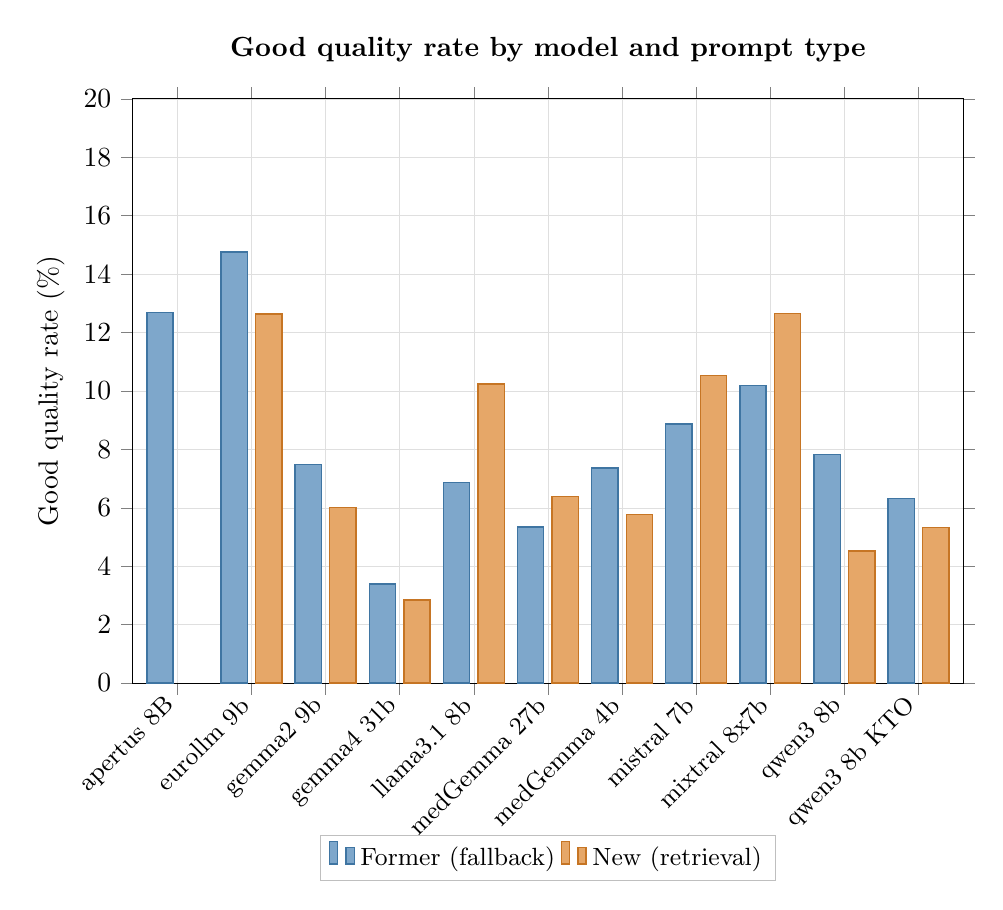
\begin{tikzpicture}
\begin{axis}[
    ybar=3pt,
    bar width=9.5pt,
    width=\textwidth,
    height=9cm,
    legend style={
        at={(0.5,-0.26)},
        anchor=north,
        legend columns=2,
        font=\small,
        draw=gray!50,
    },
    ylabel={Good quality rate (\%)},
    xtick={0,1,2,3,4,5,6,7,8,9,10},
    xticklabels={
        apertus 8B,
        eurollm 9b,
        gemma2 9b,
        gemma4 31b,
        llama3.1 8b,
        medGemma 27b,
        medGemma 4b,
        mistral 7b,
        mixtral 8x7b,
        qwen3 8b,
        qwen3 8b KTO
    },
    x tick label style={rotate=45, anchor=east, font=\small},
    ymin=0, ymax=20,
    enlarge x limits=0.06,
    grid=major,
    grid style={line width=.2pt, draw=gray!25},
    tick align=outside,
    title={Good quality rate by model and prompt type},
    title style={font=\normalsize\bfseries, yshift=4pt},
]

%% Blue bars = Former (fallback)
\addplot[
    fill=fallbackblue!70,
    draw=fallbackblue!90!black,
    line width=0.5pt,
] coordinates {
    (0,  12.68)
    (1,  14.76)
    (2,   7.48)
    (3,   3.39)
    (4,   6.86)
    (5,   5.35)
    (6,   7.37)
    (7,   8.87)
    (8,  10.19)
    (9,   7.82)
    (10,  6.32)
};

%% Orange bars = New (retrieval) — apertus 8B missing
\addplot[
    fill=retrievalorange!70,
    draw=retrievalorange!90!black,
    line width=0.5pt,
] coordinates {
    (1,  12.64)
    (2,   6.02)
    (3,   2.84)
    (4,  10.24)
    (5,   6.38)
    (6,   5.77)
    (7,  10.54)
    (8,  12.65)
    (9,   4.52)
    (10,  5.33)
};

\legend{Former (fallback), New (retrieval)}
\end{axis}
\end{tikzpicture}
\caption{Good quality rate per model and prompt type.
\textit{apertus}~8B has no retrieval-prompt data ($n=1\,096$ evaluations).}
\label{fig:grouped-bar}
\end{figure}

%% ============================================================
%% Figure 2: Delta + KTO focus (side by side)
%% ============================================================
\begin{figure}[p]
\centering

%% ---- Left sub-figure: Deltas ----
\begin{subfigure}[b]{0.60\textwidth}
\centering
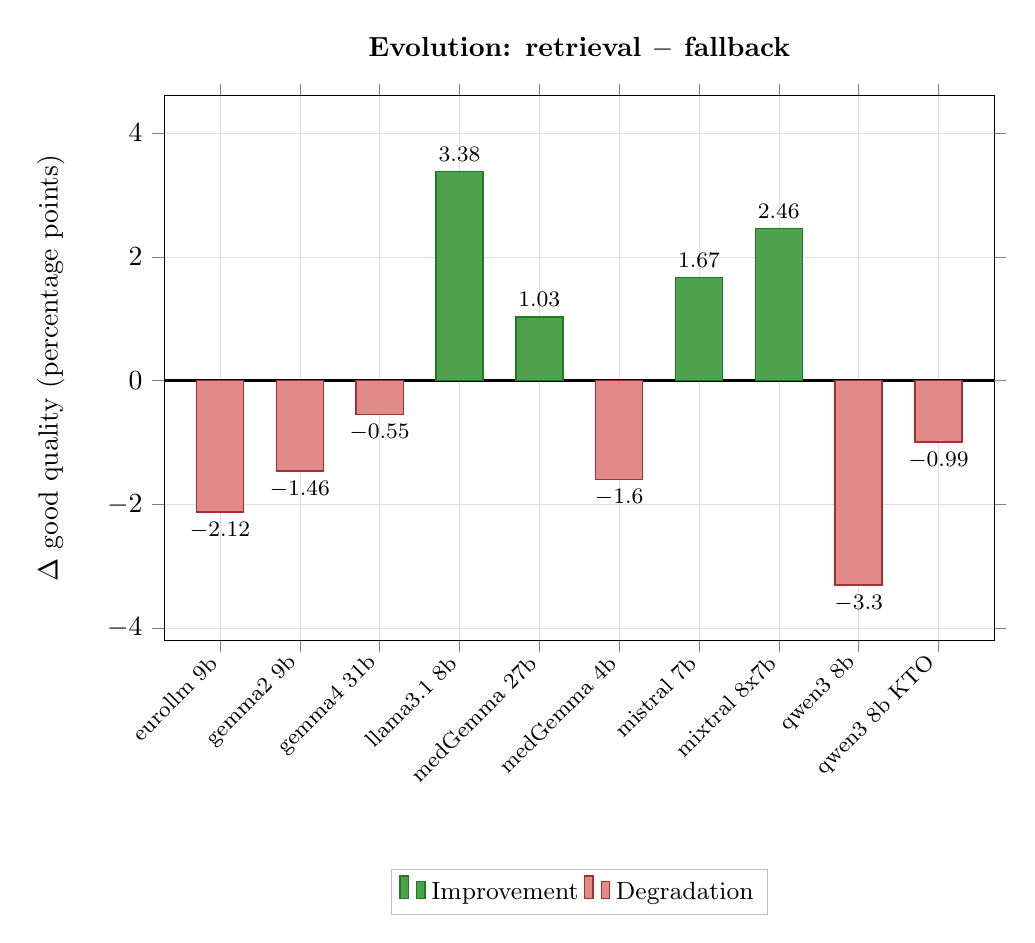
\begin{tikzpicture}
\begin{axis}[
    ybar,
    bar width=17pt,
    width=\textwidth,
    height=8.5cm,
    ylabel={$\Delta$ good quality (percentage points)},
    xtick={1,2,3,4,5,6,7,8,9,10},
    xticklabels={
        eurollm 9b,
        gemma2 9b,
        gemma4 31b,
        llama3.1 8b,
        medGemma 27b,
        medGemma 4b,
        mistral 7b,
        mixtral 8x7b,
        qwen3 8b,
        qwen3 8b KTO
    },
    x tick label style={rotate=45, anchor=east, font=\footnotesize},
    ymin=-4.2, ymax=4.6,
    xmin=0.3, xmax=10.7,
    grid=major,
    grid style={line width=.2pt, draw=gray!25},
    extra y ticks={0},
    extra y tick style={
        grid=major,
        grid style={black, line width=1.2pt},
        tick label style={draw=none},
    },
    extra y tick labels={},
    nodes near coords,
    nodes near coords align={vertical},
    every node near coord/.append style={font=\footnotesize},
    tick align=outside,
    legend style={
        at={(0.5,-0.42)},
        anchor=north,
        legend columns=2,
        font=\small,
        draw=gray!50,
    },
    title={Evolution: retrieval $-$ fallback},
    title style={font=\normalsize\bfseries, yshift=4pt},
]

%% Positive bars (improvement)
\addplot[
    fill=posgreen!80,
    draw=posgreen!90!black,
    line width=0.5pt,
    bar shift=0pt,
] coordinates {
    (4,  3.38)
    (5,  1.03)
    (7,  1.67)
    (8,  2.46)
};
\addlegendentry{Improvement}

%% Negative bars (degradation)
\addplot[
    fill=negred!60,
    draw=negred!80!black,
    line width=0.5pt,
    bar shift=0pt,
] coordinates {
    (1, -2.12)
    (2, -1.46)
    (3, -0.55)
    (6, -1.60)
    (9, -3.30)
    (10,-0.99)
};
\addlegendentry{Degradation}

\end{axis}
\end{tikzpicture}
\caption{Delta in percentage points (retrieval $-$ fallback).\\
\textcolor{posgreen}{\textbf{Green}}: improvement;
\textcolor{negred}{\textbf{Red}}: degradation.}
\label{fig:delta}
\end{subfigure}
\hfill
%% ---- Right sub-figure: KTO focus ----
\begin{subfigure}[b]{0.37\textwidth}
\centering
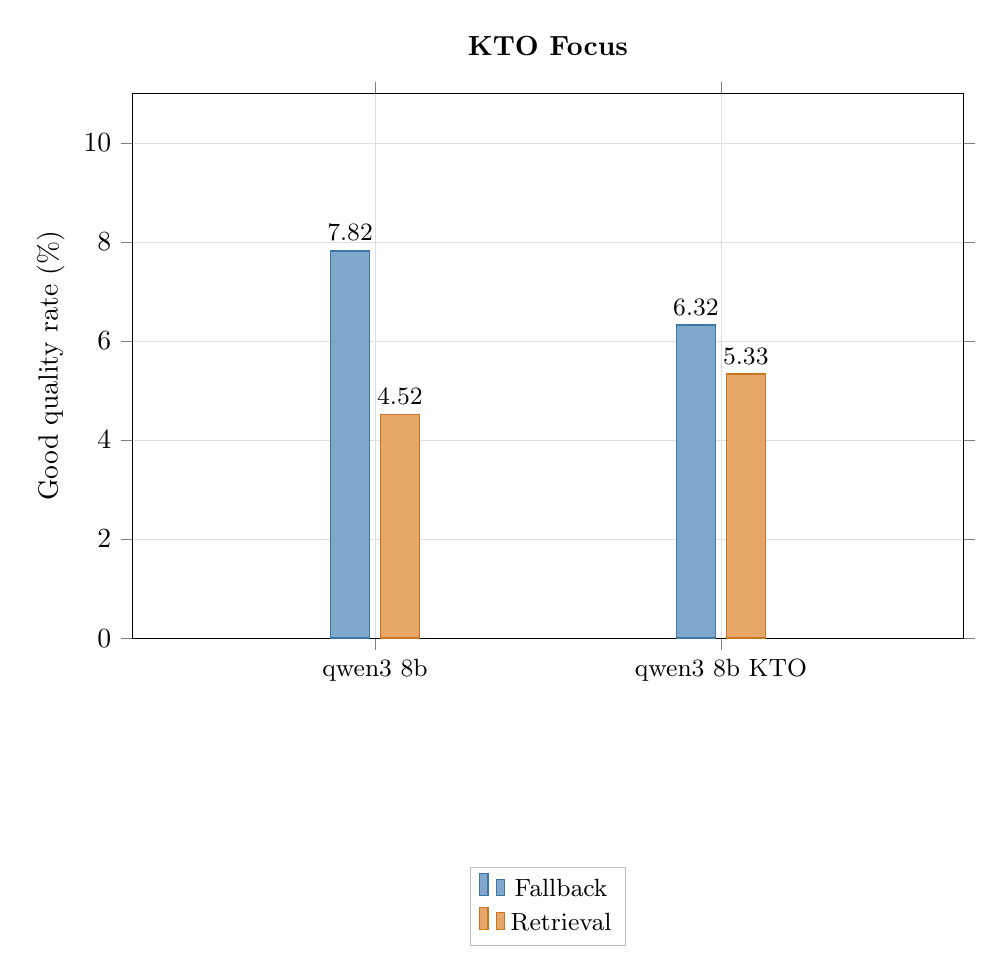
\begin{tikzpicture}
\begin{axis}[
    ybar=4pt,
    bar width=14pt,
    width=\textwidth,
    height=8.5cm,
    legend style={
        at={(0.5,-0.42)},
        anchor=north,
        legend columns=1,
        font=\small,
        draw=gray!50,
    },
    ylabel={Good quality rate (\%)},
    xtick={0,1},
    xticklabels={qwen3 8b, qwen3 8b KTO},
    x tick label style={font=\small},
    ymin=0, ymax=11,
    xmin=-0.7, xmax=1.7,
    nodes near coords,
    nodes near coords align={vertical},
    every node near coord/.append style={font=\small},
    grid=major,
    grid style={line width=.2pt, draw=gray!25},
    tick align=outside,
    title={KTO Focus},
    title style={font=\normalsize\bfseries, yshift=4pt},
]

\addplot[
    fill=fallbackblue!70,
    draw=fallbackblue!90!black,
    line width=0.5pt,
] coordinates {
    (0, 7.82)
    (1, 6.32)
};

\addplot[
    fill=retrievalorange!70,
    draw=retrievalorange!90!black,
    line width=0.5pt,
] coordinates {
    (0, 4.52)
    (1, 5.33)
};

\legend{Fallback, Retrieval}
\end{axis}
\end{tikzpicture}
\caption{Base model vs.\ KTO fine-tuned variant by prompt type.}
\label{fig:kto}
\end{subfigure}

\caption{Left: change in good quality rate (retrieval~$-$~fallback) per model
(excluding \textit{apertus}~8B, not evaluated under retrieval).
Right: focus on \textit{qwen3}~8b and its KTO variant.}
\label{fig:delta-kto}
\end{figure}

\end{document}
